
\section{Results}
\begin{table}
\centering
\begin{tabular}{ | c | c | c | c | }
	\hline
	\multicolumn{2}{|c|}{Project} & \multicolumn{2}{|c|}{Owner} \\ \hline
	Ranking & Followers & Ranking & Followers \\ \hline
	1 & 30,229 & 111,278 & 2 \\ \hline
	2 & 28,594 & 193,670 & 0 \\ \hline
	3 & 24,682 & >1,000 & -  \\ \hline
	4 & 23,830 & 21 & 4,161 \\ \hline
	5 & 22,167 & 193,670 & 0 \\ \hline
	6 & 21,227 & 111,278 & 2 \\ \hline
	7 & 17,485 & 12 & 5,213 \\ \hline
	8 & 16,543 & >1,000 & - \\ \hline
	9 & 15,648 & 87 & 1,406 \\ \hline
	10 & 15,235 & 33,877 & 12 \\ \hline
\end{tabular}
\caption{Relation between followers of a project (stars) and followers of the owner of the project. }
\label{tbl:owner}
\end{table}
\label{sec:results}

To answer Q2, we formulated four hypotheses in an attempt to characterize the motivations behind developers following a project. The hypotheses are: (i) popularity grows because the owner of the project is popular; (ii) popularity grows because the number of popular contributors working on it; (iii) popularity is affected by the programming language; (iv) popularity is determined by the category that it belongs to. We now present the results obtained for each of the four hypotheses:

\subsection{Owner}

The owner of the project is the user who originally created and published it on GitHub. We hypothesize that the popularity of the owner influences the popularity of the project he/she owns. A relation was made between the number of stars of the project and the number of followers of the owner. We started by analyzing the behaviour of the 100 most popular projects and their owners, hoping to find a positive correlation. Table \ref{tbl:owner} shows no concrete evidence about the 10 most popular projects. We could not find information about some of the owners in our database (rows 3 and 8), thus we can only affirm that they are not between the 1,000 most popular users (see Section \ref{sec:collection} for details).

A more general case is shown in Figure \ref{fig:owner}. It can be seen that a large number of popular projects have owners with little following. Finally, for the complete set of projects included in our sample, the correlation between owners and projects is 0.01, using Pearson's correlation coefficient. Therefore, we conclude that there is no correlation at all between stars and followers.
\begin{figure}
	\centering
	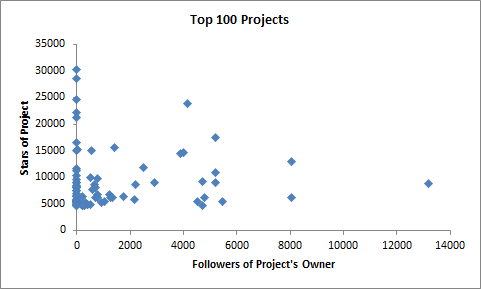
\includegraphics[width=0.45\textwidth]{./img/top100Owner.png}
	\caption{Relation between popularity of the project (given by stars) and the popularity of the project's owner (given by followers).}
	\label{fig:owner}
\end{figure}

\subsection{Contributors}

A contributor of a project is a user who actively participates in its development. We hypothesize that the involvement of one or more popular users on a project will influence on the project's popularity. In order to prove/disprove this, we collected the UserID of all contributors that belong to some of most popular projects. Due to the large amount of information and API restrictions, we could only collect the contributors of the one thousand most popular projects. We wanted to know how many popular users were contributing to such projects.

Table \ref{tbl:contributors} shows the relation between contributors and popularity of projects. We grouped the 100 and 1,000 most popular users and projects and determined the involvement of each. It shows, for example, that only 48 of the top 100 users are involved in the top 100 projects. Even more interesting, these 48 users are working on 18 of such projects. In other words, 82\% of the 100 most popular projects have no involvement of popular users. On the other side of the table, we have that almost a half (43\%) of the 1K most popular users are contributing to a quarter (22\%) of the 1K most popular projects. Because there's a large number of projects with no involvement of popular users, we dismiss this hypothesis as well.
\begin{table}
\centering
\begin{tabular}{ | l | c | c | c | c | }
	\hline
	\- & \multicolumn{2}{|c|}{Top 100 Projects} & \multicolumn{2}{|c|}{Top 1K Projects} \\ \hline
	\multicolumn{1}{|c|}{Users} & Uq Proj. & Uq Users & Uq Proj. & Uq Users \\ \hline
	Top 100 & 18 & 48 & 113 & 65 \\ \hline
	Top 1K & 23 & 286 & 222 & 431 \\ \hline
\end{tabular}
\caption{Relation between contributors and popularity of a project. Uq stands for Unique.}
\label{tbl:contributors}
\end{table}

\subsection{Programming language}

The programming language of a project can be a difficult choice for the owner. The owner probably wants to appeal to a broad audience by choosing a popular language. But sometimes there is no choice and the language is given by the specification of the project. For example, an Android app will have to be written with Java. For hypothesis 3, we wanted to determine the impact in popularity for choosing a specific programming language. We observed 128 different programming languages on our sample and a ``None'' language, which basically means that the project is missing that information. The metric we used for validating the hypothesis was the percentage of projects written in the same language that have more than 2,500 followers, a metric which we call the language success rate. We note that 2,500 followers is slightly lower than the average number of followers for the 1K most popular projects (See Table \ref{tbl:toprepos}), so we consider it a good popularity threshold.

The results are given in Table \ref{tbl:languages}. The total number of projects is given by P. F/P is the average number of followers per language and F > {$ \tau $} is the number of projects that have more than {$ \tau $} ({$ \tau $} = 2,500) followers. The last column is the language success rate. Several observations can be made. First, the two languages with the most projects (Javascript and Ruby) are also the ones that have the most projects above the {$ \tau $} threshold. Julia has a 50\% success rate, but its sample size is too little to make a reasonable generalization. Finally, the languages with a high average on followers are CSS, Rust, Julia and TypeScript, which are also the ones that have the highest success rate.

The correlation within the number of projects and the success rate is of 0.53, when the ``None'' language is removed. If we consider the ``None'' language, this correlation falls to 0.27. This tells us that there is some correlation between the most popular programming languages and the amount of projects that the language will have above the threshold {$ \tau $}. The only problem is that the success rates are so low or, in the case of Julia, the sample size is so little, that no positive conclusion can be made about the programming languages. So we also dismiss this hypothesis.
\begin{table}
\centering
\begin{tabular}{ | l | c | c | c | c | }
	\hline
	\multicolumn{1}{|c|}{Language} & P & F/P & F > {$ \tau $} & (F > {$ \tau $}) / P \\ \hline
	None & 171,894 & 1.89 & 3 & 0.002\% \\ \hline
	C & 39,716 & 8.55 & 15 & 0.038\% \\ \hline
	C\# & 15,240 & 7.84 & 1 & 0.007\% \\ \hline
	C++ & 26,071 & 7.49 & 5 & 0.019\% \\ \hline
	Clojure & 4,407 & 12.94 & 1 & 0.023\% \\ \hline
	CoffeeScript & 1,427 & 40.40 & 3 & 0.210\% \\ \hline
	CSS & 1,857 & 74.27 & 11 & 0.592\% \\ \hline
	Java & 57,953 & 6.76 & 11 & 0.019\% \\ \hline
	JavaScript & 106,987 & 17.40 & 107 & 0.100\% \\ \hline
	Julia & 2 & 1,780.00 & 1 & 50.000\% \\ \hline
	Objective-C & 20,784 & 21.87 & 21 & 0.101\% \\ \hline
	Perl & 43,808 & 2.72 & 1 & 0.002\% \\ \hline
	PHP & 54,337 & 8.39 & 12 & 0.022\% \\ \hline
	Python & 71,942 & 9.46 & 24 & 0.033\% \\ \hline
	Ruby & 173,960 & 8.89 & 51 & 0.029\% \\ \hline
	Rust & 62 & 76.18 & 1 & 1.613\% \\ \hline
	Shell & 14,158 & 9.68 & 7 & 0.049\% \\ \hline
	TypeScript & 92 & 99.39 & 1 & 1.087\% \\ \hline
	VimL & 13,961 & 9.31 & 8 & 0.057\% \\ \hline
\end{tabular}
\caption{Relation between programming languages and popularity of a project. The value chosen for {$ \tau $} was 2,500.}
\label{tbl:languages}
\end{table}
\subsection{Categories}
Our final hypothesis involves the categorization of projects. We claim that developers follow a project based on its intended usage. So, for example, 3D rendering software will usually have more followers than unit testing tools. We took the 100 most popular projects and visited their websites and repositories in order to find what their functionality is. We then assigned a broad category which we thought best described the project. The results are shown in Figure \ref{fig:categories}. We included the programming language as well, in order to better understand the distribution of the projects.

The most common categories are framework and widget / plugin. Examples of frameworks are JQuery and Symphony. Examples of widgets / plugins are FileUploader and JavaScript PDF reader. Also noteworthy to mention is that JavaScript frameworks and widgets / plugins are, by far, the most common types of project found on this phase of the study. Other categories found were front-end generators, libraries and networking tools. We believe this shows a trend about what kind of projects are users interested in following, i.e. web development productivity tools. This certainly shows the best results out of the four hypotheses we made. But, because the sample size is so small, we cannot generalize these results. In order to claim with some level of certainty that these categories correlate to the popularity of a project, we need to determine, out of all the frameworks hosted on GitHub, the percentage of successful ones. In other words, we suggest applying the same success rate metric we used for evaluating the programming languages.
\begin{figure*}[ht]
	\centering
	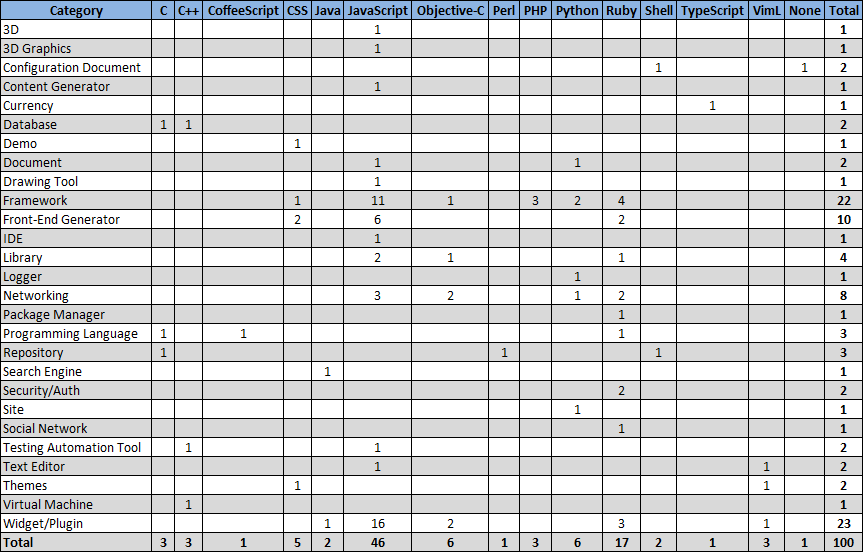
\includegraphics[width=\textwidth]{./img/categories.png}
	\caption{Categories of the 100 most popular projects, grouped by programming language. The most popular category is Widget/Plugin and 16 out of the 23 projects that fall within this category are developed using Javascript.}
	\label{fig:categories}
\end{figure*}
